\documentclass{article}

%other packages
\usepackage[a4paper]{geometry}
\usepackage{longtable}
\usepackage{wrapfig}
\setlength\parindent{0pt}
\usepackage{enumitem}
\usepackage[table]{xcolor}
\usepackage{polynom}
\def\scaleint#1{\vcenter{\hbox{\scaleto[3ex]{\displaystyle\int}{#1}}}}
\usepackage{array}
\newcolumntype{C}{>{{}}c<{{}}} % for '+' and '-' symbols
\newcolumntype{R}{>{\displaystyle}r} % automatic display-style math mode 
\usepackage{tabularray}
\usepackage{dcolumn,tabularx,booktabs}
\usepackage[most]{tcolorbox}

%maths
\usepackage{mathtools}
\usepackage{amsmath}
\usepackage{amssymb}
\usepackage{amsfonts}
\usepackage{autobreak}

%tikzpicture
\usepackage{tikz}
\usepackage{scalerel}
\usepackage{pict2e}
\usepackage{tkz-euclide}
\usepackage{tikz-3dplot}
\usetikzlibrary{calc}
\usetikzlibrary{patterns,arrows.meta}
\usetikzlibrary{shadows}
\usetikzlibrary{external}
\usetikzlibrary{decorations.pathreplacing,angles,quotes}

%pgfplots
\usepackage{pgfplots}
\pgfplotsset{compat=1.18}
\usepgfplotslibrary{statistics}
\usepgfplotslibrary{fillbetween}

\pgfplotsset{
    standard/.style={
    axis line style = thick,
    trig format=rad,
    enlargelimits,
    axis x line=middle,
    axis y line=middle,
    enlarge x limits=0.15,
    enlarge y limits=0.15,
    every axis x label/.style={at={(current axis.right of origin)},anchor=north west},
    every axis y label/.style={at={(current axis.above origin)},anchor=south east}
    }
}

\begin{document}

Math 115 - Week 2, Class 5 - 12 Jan 2024
\hrule

\vspace{10pt}

At the beginning of class, one of our classmates asked about defining an inverse for a non one-to-one function. The way to do this is to define an inverse function for each interval where the original function is one-to-one.

\begin{center}
\begin{tikzpicture}
\begin{axis}[
standard,
xmin=-3, xmax=3,
ymin=-3, ymax=3,
xtick={\empty}, ytick={\empty},
xlabel={$x$}, ylabel={$y$}]
\addplot[samples=500,domain=-4:4]{x^3-3*x} node[pos=0.566,above right]{$f$};
\draw[dashed] (-1,0) -- (-1,2);
\draw[dashed] (1,0) -- (1,-2);
\fill[] (-1,2) circle [radius=0.07];
\fill[] (1,-2) circle [radius=0.07];
\node[above] at (-1,2) {$a$};
\node[below] at (1,-2) {$b$};
\end{axis}
\end{tikzpicture}
\end{center}

\[D=(-\infty,a]\cup(a,b]\cup(b,\infty)\]

This particular function is one-to-one on three intervals, so we would define an inverse for each and it would be understood from the context of future questions which one should be used.

\vspace{10pt}

After answering the question, we moved on to some differentiation and integration of exponential and logarithmic functions.

\begin{center}
\begin{tabular}{|ll|}
\hline&\\
$(e^x)^\prime=e^x$ & So, $\int e^x\ dx=e^x+C$\\[1em]
$(a^x)^\prime=a^x\ln a$ & So, $\int a^x\ dx=\frac{a^x}{\ln a}+C$\\[1em]
\hline
\end{tabular}
\end{center}

At this point, we differentiated the natural logarithmic function, making use of the fact that the derivatives of a function is the same as the reciprocal of the derivative of its inverse.

\begin{center}
$\boxed{\begin{gathered}
\frac{dy}{dx}=\frac{1}{\left(\frac{dx}{dy}\right)}
\end{gathered}}$
\end{center}

So,

\begin{align*}
\textnormal{Let }y&=\ln x\\
x&=e^y\\
\frac{dx}{dy}&=e^y=x\\
\therefore(\ln x)^\prime&=\frac{1}{x}
\end{align*}

Reversing this logic, we can now obtain the indefinite integral of the reciprocal function for all $x>0$.

\[\int\frac{1}{x}\ dx\textnormal{ where } x>0=\ln x+C\]

And by using a substitution, we can obtain the indefinite integral of the reciprocal function for all $x<0$.

\[\textnormal{Let }t=-x,\ dt=-dx\Rightarrow\int\frac{1}{t}\ dt=\ln t+C\]

Therefore,

\[\int\frac{1}{x}\ dx\textnormal{ where } x<0=\ln x+C\]

We then recalled the piecewise definition of the absolute value function.

\[|x|=\left\{\begin{array}{rl}x&\textnormal{if }x\geq0\\-x&\textnormal{if }x<0\end{array}\right.\]

And applied it to our definition of the indefinite integral of the reciprocal function.

\begin{center}
\begin{tabular}{|rl|}
\hline&\\
$\displaystyle\int\frac{1}{x}\ dx$ & $=\left\{\begin{array}{rl}\ln x+C&\textnormal{if }x>0\\\ln(-x)+C&\textnormal{if }x<0\end{array}\right.$\\[1.5em]
& $\displaystyle=\ln|x|+C$\\[1em]
\hline
\end{tabular}
\end{center}

When it comes to examinations, use this formula because we were taught it in class. That being said, the formula is actually incorrect, as I pointed out in class. Since it is beyond the scope of the course, I will not demonstrate this fact here, but if you're interested in discovering the truth of the matter, A Mathematician from the Univerity of Victoria, Dr. Trefor Bazett, published a very nice Youtube video explaining it. The video is called "Your calculus prof lied to you (probably)".

\vspace{10pt}

Anyways, back to the course material. Using the change of base formula in addition to what we have just discussed, we can easily arrive at the derivative of a logarithm of arbitrary positive base.

\begin{center}
\begin{tabular}{|rl|}
\hline&\\
$\log_ax$ & $=\frac{\ln x}{\ln a}$\\[0.5em]
$(\log_ax)^\prime$ & $=\frac{1}{\ln a}\cdot\frac{1}{x}$\\[1em]
\hline
\end{tabular}
\end{center}

After this, we spent some time in class solving exercises.

\vspace{10pt}

{\bf{}EXAMPLE} Evaluate $\displaystyle\lim_{x\to\infty}e^{-x^2}$

\[\lim_{x\to\infty}e^{-x^2}=\left(\begin{array}{rl}-x^2&=t\\t&\to-\infty\end{array}\right)=\lim_{t\to-\infty}e^t=0+\]

\vspace{10pt}

{\bf{}EXAMPLE} Evaluate $\displaystyle\lim_{x\to2^-}e^\frac{3}{2-x}$

\[\textnormal{Let }2-x=t\Rightarrow x=2-t\]

So,

\begin{align*}
\lim_{x\to2^-}e^\frac{3}{2-x}&=\left(\begin{array}{rl}x&\to2^-\\t&\to-0^+\end{array}\right)\\
&=\lim_{t\to0^+}e^\frac{3}{t}\\
&=+\infty
\end{align*}

{\bf{}EXAMPLE} Evaluate $\displaystyle\lim_{x\to\frac{\pi}{2}^+}e^{\tan x}$

\vspace{10pt}

To answer this question, it may be useful to recall the geometric (unit circle) definitions of the trigonometric functions.

\vspace{10pt}

Let $s=\sin\theta,\ c=\cos\theta,\ t=\tan\theta$

\begin{center}
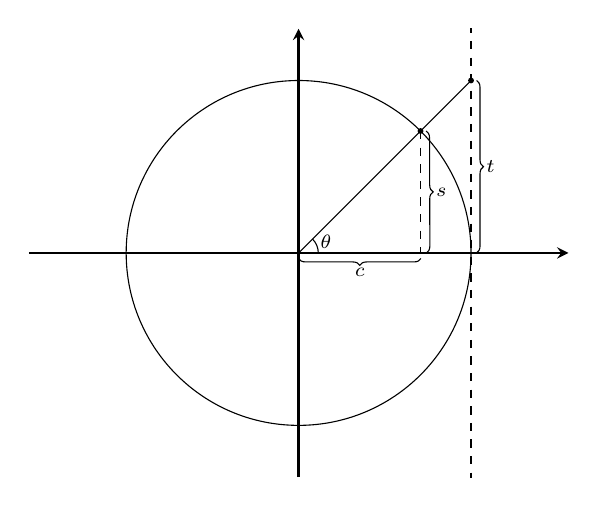
\begin{tikzpicture}
\begin{axis}[standard,
xmin=-1, xmax=1,
ymin=-1, ymax=1,
axis equal,
trig format=deg,
xtick={\empty}, ytick={\empty}]
\draw[] (0,0) circle [radius=1];
\draw[] (0,0) -- (45:1);
\fill[] (45:1) circle [radius=0.017];
\draw[dashed] (45:1) |- (0,0);
\draw[decoration={brace,mirror,raise=2pt},decorate] (1/1.41,0) -- (45:1) node[pos=0.5,right=2pt]{$\scriptstyle s$};
\draw[decoration={brace,mirror,raise=2pt},decorate](0,0) -- (1/1.41,0) node[pos=0.5,below=2pt]{$\scriptstyle c$};
\coordinate (O) at (0,0);
\coordinate (P) at (45:1);
\coordinate (X) at (45:1 |- 0,0);
\draw[] pic["$\scriptstyle\theta$",-,angle eccentricity=1.5, angle radius=0.25cm,draw]{angle=X--O--P};
\draw[] (P) -- (1,1);
\fill[] (1,1) circle [radius=0.017];
\draw[dashed] (1,2) -- (1,-2);
\draw[decoration={brace,mirror,raise=2pt},decorate] (1,0) -- (1,1) node[pos=0.5,right=2pt]{$\scriptstyle t$};
\end{axis}
\end{tikzpicture}
\end{center}

So,

\[\lim_{x\to\frac{\pi}{2}^+}e^{\tan x}=\left(\begin{array}{rl}\tan x&=u\\u&\to-\infty\end{array}\right)=\lim_{u\to-\infty}e^u=0\]

\vspace{10pt}

{\bf{}EXAMPLE} Differentiate $y=e^{-2t}\cos4t$

\vspace{10pt}

This is a product and chain rule exercise.

\[y^\prime=-2e^{-2t}\cos4t-4e^{-2t}\sin4t\]

\vspace{10pt}

{\bf{}EXAMPLE} Differentiate $y=\ln(\cos3x^2)$

\vspace{10pt}

This is a chain rule exercise.

\[y^\prime=\frac{1}{\cos3x^2}\cdot(-\sin3x^2)\cdot6x\]

\vspace{10pt}

With the conclusion of the exercised, we moved onto our final theoretical point: differentiating functions where the variable is in both the exponent and the base.

\vspace{10pt}

Solution 1:

\begin{align*}
y&=x^x\\
\ln y&=x\ln x\\
\frac{1}{y}y^\prime&=1+\ln x\\
\therefore y^\prime&=x^x(\ln x+1)
\end{align*}

Solution 2:

\begin{align*}
y&=x^x\\
&=e^{\ln(x^x)}\\
&=e^{x\ln x}\\
\therefore y^\prime&=e^{x\ln x}(\ln x+1)\\
&=x^x(1+\ln x)
\end{align*}

And finally, we differentiated one function exponentiated to another.

\begin{align*}
y&=f(x)^{g(x)}\\
\ln y&=g(x)\ln f(x)\\
\frac{1}{y}y^\prime&=g^\prime(x)\ln f(x)+g(x)\cdot\frac{1}{f(x)}\cdot f^\prime(x)\\
\therefore y^\prime&=x^x[g^\prime(x)\ln f(x)+g(x)\cdot\frac{1}{f(x)}cdot f^\prime(x)]
\end{align*}



\end{document}